%&pdflatex
\documentclass[mathserif]{beamer} %, handout
\usetheme[progressbar=foot]{metropolis}
\setbeamertemplate{caption}[numbered]

\usepackage[utf8x]{inputenc}
\usepackage[T1]{fontenc}
\usepackage[english]{babel}

\usepackage{amssymb, amsmath, amsfonts, mathtools, mathrsfs}
\usepackage{comment}

\AtBeginSubsection{
\frame[plain,c]{\subsectionpage}
}

\defbeamertemplate{subsection page}{simple}{
  \centering
  \usebeamercolor[fg]{subsection title}
  \usebeamerfont{subsection title}
  \insertsubsection\\
}
\setbeamertemplate{subsection page}[simple]

\title{High-accuracy numerical solution of the Boltzmann equation}
\author{Oleg Rogozin}
\institute{
    Dorodnicyn Computing Center \\
    Federal Research Center of Computing Science and Control \\
    Russian Academy of Sciences
}
\date{}

\newcommand\pro{\item[$+$]}
\newcommand\con{\item[$-$]}

\newcommand{\Kn}{\mathrm{Kn}}
\newcommand{\Ma}{\mathrm{Ma}}
\newcommand{\dd}{\:\mathrm{d}}
\newcommand{\pder}[2][]{\frac{\partial#1}{\partial#2}}
\newcommand{\pderdual}[2][]{\frac{\partial^2#1}{\partial#2^2}}
\newcommand{\pderder}[2][]{\frac{\partial^2 #1}{\partial #2^2}}
\newcommand{\Pder}[2][]{\partial#1/\partial#2}
\newcommand{\dxi}{\boldsymbol{\dd\xi}}
\newcommand{\bxi}{\boldsymbol{\xi}}
\newcommand{\bh}{\boldsymbol{h}}
\newcommand{\be}{\boldsymbol{e}}
\newcommand{\Nu}{\mathcal{N}}
\newcommand{\OO}[1]{O(#1)}
\newcommand{\Set}[2]{\{\,{#1}:{#2}\,\}}
\newcommand{\deltann}[2]{(\delta_{#1#2}-n_#1 n_#2)}
\newcommand{\onwall}[1]{\left(#1\right)_0}
\newcommand{\xoverbrace}[2][\vphantom{\int}]{\overbrace{#1#2}}

\begin{document}

\frame{\titlepage}
% Despite of acadEmic character of my report, I sincerely hope to bring some ideas into the main direction of this workshop.

\begin{frame}
  \frametitle{Plan}
  \linespread{0.8}
  \tableofcontents
  % I will present some high-accuracy numerical examples based on the direct solution of the BE
  % and compare them with the asymptotic solutions.
\end{frame}

\section{Motivation}

\begin{frame}
    \frametitle{Motivation}
    \begin{center}
        The \alert{linear} Couette-flow problem for BGK gas [Prof. Aristov's talk]
        Discrete-velocity solution on the \alert{uniform} grid with \(N=2176\) nodes
        \vspace{-10pt}
    	\includegraphics[width=.9\textwidth]{../../reports/9_bgk_lattice/couette/dvm2}
	\end{center}
\end{frame}

\begin{frame}
    \frametitle{Motivation}
    \begin{center}
        Close-up of the velocity profile in the Knudsen layer\\
        Discontinuity at the boundary and \(\xi_in_i=0\)
        \includegraphics[width=\textwidth, clip=true, trim = 250 100 15 30 mm]%
            {../../reports/9_bgk_lattice/couette/dvm2}
    \end{center}
\end{frame}

\begin{frame}
    \frametitle{Motivation}
    \begin{center}\Large\bf
        How can we increase accuracy in the Knudsen layer?
    \end{center}
    \begin{itemize}
        \item grid refinement near discontinuity
        \begin{itemize}
            \con large computational cost
            \con \textit{ad hoc} grid
            \pro arbitrary \(\Kn\)
        \end{itemize}
        \item fluid-dynamic solution + Knudsen-layer correction (Kyoto group)
        \begin{itemize}
            \con small \(\Kn\)
            \con smooth boundary
            \pro computationally efficient
        \end{itemize}
        \item ...
    \end{itemize}
\end{frame}

\section{Numerical analysis}

\begin{frame}
    \frametitle{Numerical methods for the nonlinear Boltzmann equation}
    \begin{columns}
		\column{.6\textwidth}
		\begin{itemize}
            \item DSMC
            \begin{itemize}
                \pro unbounded velocity space
                \con low stochastic accuracy
            \end{itemize}
            \vspace{20pt}
            \item \textbf{discrete-velocity}
            \begin{itemize}
                \pro conservative projection technique \newline [Tcheremissine 1998]
                \pro second-order accuracy
            \end{itemize}
            \only<2>{\footnotesize\alert{[Morris, Varghese, Goldstein et al. 2012]}}
        \end{itemize}
		\column{.6\textwidth}
		\begin{itemize}
            \item \textbf{discontinuous Galerkin} (polynomial, Laguerre, \dots)
            \begin{itemize}
                \pro high-order accuracy
                \con complicated % many parameters should be tuned
            \end{itemize}
            \only<2>{\alert{[Ohwada 1993]}}
            \vspace{20pt}
            \item \textbf{Fourier--Galerkin}
            \begin{itemize}
                \pro fast algorithm \newline [Mouhot, Pareschi 2006]
                \pro spectral accuracy
                \con nonconservative
                \con Gibbs phenomenon
            \end{itemize}
            \only<2>{
                {\footnotesize\alert{[Heintz, Kowalczyk, Grzhibovskis 2008]}} \\
                \alert{[Wu, Reese, Zhang 2014]}
            }
        \end{itemize}
	\end{columns}
\end{frame}

\subsection{Method for solution of the Boltzmann equation}

\begin{frame}
    \frametitle{Outline of the method}
    \vspace{-5pt}
    \begin{equation}
        \pder[f]{t} + \xi_i\pder[f]{x_i} = J(f,f)
    \end{equation}
    \vspace{-10pt}
    \begin{block}{Symmetric second-order splitting}
        \begin{equation}
            S_{A+B}^{\tau} = S_A^{\tau/2}S_B^{\tau}S_A^{\tau/2} + \OO{\tau^2}
        \end{equation}
    \end{block}
    \pause
    \begin{columns}[T]
        \begin{column}{5cm}
            \begin{block}{Collisionless BE}
                \begin{equation}
                    \pder[f]{t} + \xi_i\pder[f]{x_i} = 0
                \end{equation}
                \vspace{-15pt}
                \begin{itemize}
                    \item finite-volume method
                    \item TVD scheme \(\OO{\tau^2, h^2}\)
                    \item (un)structured grid
                \end{itemize}
            \end{block}
        \end{column}
        \begin{column}{6.5cm}
            \begin{block}{Spatially homogeneous BE}
                \begin{equation}
                    \pder[f]{t} = J(f,f)
                \end{equation}
                \vspace{-15pt}
                \begin{itemize}
                    \item projection discrete-velocity method
                    \item scheme in fractional steps \(\OO{\tau^2, h^2}\)
                    \item rectangular grid
                \end{itemize}
            \end{block}
        \end{column}
    \end{columns}
\end{frame}

\begin{frame}
    \frametitle{The discretization of the velocity space}
    Grid \(\mathcal{V} = \Set{\xi_\gamma}{\gamma\in\Gamma}\) is constructed so that
    \begin{equation}\label{eq:xi_cubature}
        \int F(\bxi) \dxi \approx \sum_{\gamma\in\Gamma} F_\gamma w_\gamma =
            \sum_{\gamma\in\Gamma} \hat{F_\gamma},
            \quad F_\gamma = F(\bxi_\gamma),
    \end{equation}\vspace{-10pt}

    where \(\sum_{\gamma\in\Gamma} w_\gamma = V_\Gamma\) is the volume of the velocity grid.
    \pause\vspace{20pt}

    The symmetrized collision integral\vspace{-20pt}

    \begin{equation}\label{eq:symm_ci}
        J(f_\gamma, f_\gamma) = \frac14\int \left(
            \delta_\gamma + \delta_{\gamma*} - \delta'_\gamma - \delta'_{\gamma*}
        \right) (f'f'_* - ff_*)B \dd\Omega(\boldsymbol{\alpha}) \dxi\dxi_*
    \end{equation}\vspace{-30pt}

    has the following discrete analogue: % quantities with accents
    \begin{equation}\label{eq:discrete_symm_ci}
        \footnotesize
        \hat{J}_\gamma = \frac{\pi V_\Gamma^2}{\displaystyle\sum_{\nu\in\Nu} w_{\alpha}w_{\beta}}
            \sum_{\nu\in\Nu} \bigg(
                \delta_{\alpha\gamma} + \delta_{\beta\gamma} -
                \xoverbrace{ \alert{\delta_{\alpha'\gamma}} - \alert{\delta_{\beta'\gamma}} }^\text{projection}
            \bigg)\bigg(
                \xoverbrace{ \frac{w_{\alpha}w_{\beta}}{\alert{w_{\alpha'}w_{\beta'}}}
                \alert{\hat{f}_{\alpha'}\hat{f}_{\beta'}} }^\text{interpolation} - \hat{f}_{\alpha}\hat{f}_{\beta}
            \bigg)B_\nu.
    \end{equation}\vspace{-10pt}
\end{frame}

\begin{frame}
    \frametitle{Conservative projection}
    \centering{\Large\bf Why the method is called as "projection"?} % why, actually, ...
    \vspace{10pt}

    Petrov--Galerkin projection method:
    \begin{equation}\label{eq:Petrov-Galerkin}
        \int \xoverbrace{ \psi_s(\bxi_\gamma) }^\text{test space} \bigg(
            \alert{\delta(\bxi'-\bxi_\gamma)} - \sum_{a\in\Lambda} r_{\lambda,a}
            \xoverbrace{ \delta(\bxi_{\lambda+s_a}-\bxi_\gamma) }^\text{trial space}
        \bigg) \dxi_\gamma = 0.
    \end{equation}
    \begin{itemize}
        \item \(r_{\lambda,a}\) are the \emph{projection weights} (in space \(\mathcal{V}\))
        \item \(\mathcal{S} = \Set{s_a}{a\in\Lambda, r_{\lambda,a}\neq0}\) is the \emph{projection stencil}
            \\ (set of displacement rules)
        \item \(\psi_0 = 1, \psi_i = \xi_i, \psi_4 = \xi_i^2\) are the \emph{collisional invariants}
        \item the same holds for \(\alert{\delta(\bxi'_*-\bxi_\gamma)}\)
    \end{itemize}
\end{frame}

\begin{frame}
    \frametitle{Interpolation of the distribution function}
    As a general example, use the weighted Kolmogorov mean: % we have many freedom to define the interpolation procedure
    \begin{equation}\label{eq:Kolmogorov_mean}
        \begin{dcases}
            \alert{\hat{f}_{\alpha'}} = \phi^{-1}_f\left(\sum_{a\in\Lambda} q_{\lambda,a}
                \phi_f\left(\hat{f}_{\lambda+s_a}\right)\right), \\
            \alert{w_{\alpha'}} = \phi^{-1}_w\left(\sum_{a\in\Lambda} p_{\lambda,a}
                \phi_w\left(w_{\lambda+s_a}\right)\right), \\
        \end{dcases}
    \end{equation}
    If we take the geometric mean
    \begin{equation}\label{eq:geometric_mean}
       \phi_{f,w}(x) = \ln(x), \quad \phi_{f,w}^{-1}(x) = \exp(x), \quad p_{\lambda,a} = q_{\lambda,a} = r_{\lambda,a},
    \end{equation}
    then \(\mathcal{H}\)-theorem holds and
    \begin{equation}\label{eq:strict_interpolation}
        \hat{J}_\gamma(\hat{f}_{M\gamma}, \hat{f}_{M\gamma}) = 0.
    \end{equation}
    The same should hold for \(\alert{w_{\beta'}}\) and \(\alert{\hat{f}_{\beta'}}\).
\end{frame}

\begin{frame}
    \frametitle{Cauchy problem for the space-homogeneous BE}
    Rewrite
    \begin{equation}
        \hat{J}_\gamma = \frac{\pi V_\Gamma^2}{\sum_{\nu\in\Nu} w_{\alpha}w_{\beta}}
        \sum_{\nu\in\Nu} \left(
            \delta_{\alpha\gamma} + \delta_{\beta\gamma} -
            \delta_{\alpha'\gamma} - \delta_{\beta'\gamma}
        \right)\big(\cdots\big)B_\nu
    \end{equation}
    as
    \begin{equation}
        \hat{J}_{\gamma} = \sum_{j=1}^N \hat{\Delta}_{\gamma}^{n+(j-1)/N}, \quad N=|\Nu|.
    \end{equation}
    Then we can build a conservative scheme in fractional steps
    \begin{equation}\label{eq:fractional_step_scheme}
        \hat{f}_\gamma^{n+j/N} = \hat{f}_\gamma^{n+(j-1)/N} + \frac{t_{n+1}-t_n}{N}\hat{\Delta}_{\gamma}^{n+(j-1)/N}
        \quad (j = 1,\dotsc,N).
    \end{equation}
    \begin{itemize}
        \item every \(\hat{\Delta}_{\gamma}^{n+(j-1)/N}\) contains \(2(1+|\mathcal{S}|)\) nonzero elements
        \item every fractional step preserve mass, momentum, energy
    \end{itemize}
\end{frame}

\begin{frame}
    \frametitle{Positivity of the distribution function}
    To ensure positivity in practice, some cubature points (say, \(\mathcal{M}\)) can be excluded:
    \begin{equation}\label{eq:discrete_short_ci_discarded}
        \hat{J}_\gamma = \sum_{\nu\in\Nu\alert{\setminus\mathcal{M}}} \hat{\Delta}_{\gamma\nu}.
    \end{equation}
    \vspace{10pt}

    \(|\Nu|\) is adapted to control a smallness of the excluded-points contribution in each physical cell:
    \begin{equation}\label{eq:excluded_contribution}
        \frac{\sum_{\nu\in\mathcal{M}} \left| \hat{\Delta}_{\alpha\nu} \right|}
            {\sum_{\nu\in\Nu\setminus\mathcal{M}} \left| \hat{\Delta}_{\alpha\nu} \right|} < \varepsilon.
    \end{equation}
    Usually, \(\varepsilon \lesssim 10^{-5}\) for high-accuracy solution.
\end{frame}

\subsection{Examples of projection stencils}

\begin{frame}
    \frametitle{2-point scheme for a uniform grid}
    \begin{equation}\label{eq:discrete_symm_ci_uniform}
        J_\gamma = \frac{\pi V_\Gamma|\Gamma|}{|\Nu|}
            \sum_{\nu\in\Nu} \left(
                \delta_{\alpha\gamma} + \delta_{\beta\gamma}
                - \delta_{\alpha'\gamma} - \delta_{\beta'\gamma}
            \right)\left( f_{\alpha'} f_{\beta'} - f_{\alpha} f_{\beta} \right)B_\nu.
    \end{equation}
    \vspace{-20pt}

    Due to the symmetry of the grid, we need only two nodes:
    \begin{equation}\label{eq:uniform_projection}
        \delta_{\alpha'\gamma} = (1-r)\delta_{\lambda\gamma} + r\delta_{\lambda\alert{+s},\gamma}, \quad
        \delta_{\beta'\gamma} = (1-r)\delta_{\mu\gamma} + r\delta_{\mu\alert{-s},\gamma},
    \end{equation}
    where
    \begin{equation}\label{eq:r_uniform}
        r = \frac{E_0-E_1}{E_2-E_1}, \quad
        E_0 = \bxi_{\alpha'}^2 + \bxi_{\beta'}^2, \quad
        E_1 = \bxi_{\lambda}^2 + \bxi_{\mu}^2, \quad
        E_2 = \bxi_{\lambda+s}^2 + \bxi_{\mu-s}^2.
    \end{equation}
    \vspace{-20pt}

    Note that \(0\leq r < 1\).
\end{frame}

\begin{frame}
    \frametitle{5-point scheme for nonuniform grids}
    \begin{equation}\label{eq:eta_definition}
        \boldsymbol{\eta} = \bxi_{\alpha'} - \bxi_{\lambda}, \quad
        0 \leq \frac{\eta_i}{h^+_i} \leq \frac12, \quad
        -\frac12 \leq \frac{\eta_i}{h^-_i} \leq 0.
    \end{equation}

    \emph{Compact 5-point scheme} is constructed on the following nodes
    \begin{equation}\label{eq:stencil_nodes_5}
        \bxi_{\lambda+s_0} = \bxi_{\lambda}, \quad
        \bxi_{\lambda+s_i} = \bxi_{\lambda} + (\bh^+\cdot \be_i)\be_i, \quad
        \bxi_{\lambda+s_4} = \bxi_{\lambda} + \bh^-.
    \end{equation}

    The projection weights are calculated as
    \begin{equation}\label{eq:stencil_weights_5}
        r_{\lambda,0} = 1 - \sum_{j=1}^4 r_{\lambda,j}, \quad
        r_{\lambda,i} = \frac{\eta_i - r_{\lambda,4}h^-_i}{h^+_i}, \quad
        r_{\lambda,4} = \frac{\boldsymbol{\eta}\cdot(\boldsymbol{\eta} - \bh^+)}
            {\bh^-\cdot(\bh^- - \bh^+)}.
    \end{equation}
    \vspace{-20pt}

    For the uniform grid, the following estimates hold
    \begin{equation}\label{eq:weights_ranges_5}
        0 \leq r_{\lambda,0} \leq 1, \quad
        -\frac1{12} \leq r_{\lambda,i} \leq \frac{11}{24}, \quad
        -\frac18 \leq r_{\lambda,4} \leq 0, \quad
        R_\mathcal{S} = \sqrt{6}.
    \end{equation}
\end{frame}

\begin{frame}
    \frametitle{7-point scheme for nonuniform grids}
    \emph{Symmetric 7-point circuit} is constructed on the following nodes
    \begin{equation}\label{eq:stencil_nodes_7}
        \bxi_{\lambda+s_0} = \bxi_{\lambda}, \quad
        \bxi_{\lambda+s_{\pm i}} = \bxi_{\lambda} + (\bh^\pm\cdot \be_i)\be_i.
    \end{equation}

    The projection weights are calculated as
    \begin{equation}\label{eq:stencil_weights_7}
        r_{\lambda,0} = 1 - \sum_{j=1}^3 r_{\lambda,j} + r_{\lambda,-j}, \quad
        r_{\lambda,\pm i} = \pm\frac{\eta_i(\eta_i - h^\mp_i)}{h^\pm_i(h^+_i-h^-_i)}.
    \end{equation}

    For the uniform grid, the following estimates hold
    \begin{equation}\label{eq:weights_ranges_7}
        \frac14 \leq r_{\lambda,0} \leq 1, \quad
        0 \leq r_{\lambda,\pm i} \leq \frac38, \quad
        -\frac18 \leq r_{\lambda,\mp i} \leq 0, \quad
        R_\mathcal{S} = 2.
    \end{equation}
\end{frame}

\section{Asymptotic analysis}
\subsection{Nonisothermal slow flows}

\begin{frame}
    \frametitle{Hilbert expansion for slow flows}
    The stationary Boltzmann equation in the presence of an external force
    \begin{equation}\label{eq:Boltzmann}
        \xi_i\pder[f]{x_i} + F_i\pder[f]{\xi_i} = \frac1k J(f,f).
    \end{equation}
    The expansion in the Knudsen number \(k=\Kn\sqrt\pi/2\):
    \begin{equation}\label{eq:expansion}
        f = f_0 + f_1k + f_2k^2 + \cdots, \quad h = h_0 + h_1k + h_2k^2 + \cdots,
    \end{equation}
    where the macroscopic quantities \(h = \rho, v_i, T, \dots\)
    \vspace{5pt}\pause

    Assumptions:
    \begin{itemize}
        \item slow flows \(\int\xi_i f\dxi = v_i = \OO{k}\) (\(\mathrm{Re} = \OO{1}\))
        \item weak external force \(F_i = \OO{k^2}\)
    \end{itemize}
    Due to the degeneracy of the momentum equation,
    \begin{equation}
        \pder[p_0]{x_i} = 0, \quad \pder[p_1]{x_i} = 0.
    \end{equation}
\end{frame}

\begin{frame}
    \frametitle{Kogan--Galkin--Friedlander equations [KGF 1976]}
    The notation follows [Sone 2007]
    \begin{align}
        \pder{x_i}\left(\frac{u_{i1}}{T_0}\right) &= 0, \label{eq:asymptotic1} \\
        \pder{x_j}\left(\frac{u_{i1}u_{j1}}{T_0}\right)
            &-\frac{\gamma_1}2\pder{x_j}\left[\sqrt{T_0}\left(
                \pder[u_{i1}]{x_j} + \pder[u_{j1}]{x_i} - \frac23\pder[u_{k1}]{x_k}\delta_{ij}
            \right)\right] \notag\\
            &\alert{- \frac{\bar{\gamma}_7}{T_0}\pder[T_0]{x_i}\pder[T_0]{x_j}
                \left(\frac{u_{j1}}{\gamma_2\sqrt{T_0}} - \frac{1}4\pder[T_0]{x_j}\right)} \notag\\
            &= -\frac12\pder[p_2^\dag]{x_i} + \frac{p_0^2 F_{i2}}{T_0}, \label{eq:asymptotic2} \\
        \pder[u_{i1}]{x_i} &= \frac{\gamma_2}2\pder{x_i}\left(\sqrt{T_0}\pder[T_0]{x_i}\right), \label{eq:asymptotic3}
    \end{align}
    where
    \begin{equation}\label{eq:dag_pressure}
        p_2^\dag = p_0 p_2
            + \frac{2\gamma_3}{3}\pder{x_k}\left(T_0\pder[T_0]{x_k}\right)
            - \frac{\bar{\gamma}_7}{6}\left(\pder[T_0]{x_k}\right)^2, \quad u_{i1} = p_0v_{i1}.
    \end{equation}
\end{frame}

\begin{frame}
    \frametitle{Acting forces \(\OO{k^2}\)}
    The force acting on the unit of mass of the gas is
    \begin{equation}\label{eq:gamma7_force}
        F_{i2} = \frac{\bar{\gamma}_7}{p_0^2}\pder[T_0]{x_i}\pder[T_0]{x_j}\left(\frac{u_{j1}}{\gamma_2\sqrt{T_0}}
            - \frac{1}4\pder[T_0]{x_j}\right).
    \end{equation}
    It causes the \alert{nonlinear thermal-stress flow}.
    For a hard-sphere gas, \(\bar{\gamma}_7 = \gamma_3 - \gamma_7 = 1.758705\).
    \vspace{20pt}\pause

    The force acting on a uniformly heated body at rest is
    \begin{multline}\label{eq:force:terms}
        p_0 \oint_S F_{i2} \dd{S} =
            - \overbrace{ \oint_S p_2^\dag n_i \dd{S} }^\text{pressure} \\
            + \underbrace{ \gamma_1 \sqrt{T_{B0}} \oint_S \pder[u_{i1}]{x_j} n_j \dd{S} }_\text{viscosity}
            + \underbrace{ \frac{\bar{\gamma}_7}{2} \oint_S \left(\pder[T_0]{x_j}\right)^2 n_i \dd{S} }_\text{thermal-stress}.
    \end{multline}
\end{frame}

\begin{frame}
    \frametitle{Boundary conditions and Knudsen-layer correction}
    Both are taken from the \alert{high-accuracy} solution of the 1D half-space problems.
    \begin{itemize}
        \item first order [Ohwada, Sone, Aoki 1989]
        \item second order [Takata, Hattori 2015]
    \end{itemize}
    \vspace{10pt}
    \pause

    The macroscopic variables \(h = h_0 + (h_1 + \alert{h_{K1}})k + \cdots\)

    Rigorous theorems [Maslova 1982; Bardos, Caflisch, Nicolaenko 1986]:
    \begin{equation}
        h_K = \OO{e^{-\lambda\eta}}, \quad \eta = \frac{p_0}{T_{B0}}(x_i-x_{Bi})\frac{n_i}k
    \end{equation}
\end{frame}

\subsection{Plane Prandtl layer}

\begin{frame}
    \frametitle{Hilbert expansion for a plane one-dimensional flow}
    \begin{equation}\label{eq:Hilbert_plane_1d}
        \xi_y\pder[f]{y} = \frac1k J(f,f), \quad v_x = (u, 0, 0).
    \end{equation}
    \pause
    Navier--Stokes equations:
    \begin{gather}
        \pder{y}\left( \sqrt{T_0}\pder[u_0]{y} \right) = \OO{\alert{k^2}}, \\
        \sqrt{T_0}\left( \pder[u_0]{y}\right)^2 + \frac{5\gamma_2}
            {4\gamma_1}\pder{y}\left(\sqrt{T_0}\pder[T_0]{y} \right) = \OO{\alert{k^2}}.
    \end{gather}
    Slip/jump boundary conditions:
    \begin{equation}
        u = u_B + b_1\frac{T_0}{p_0} \pder[u_0]{y}k + \OO{\alert{k^2}}, \quad
        T = T_B + c_1\frac{T_0}{p_0}\pder[T_H]{y}k + \OO{\alert{k^2}}.
    \end{equation}
\end{frame}

\begin{frame}
    \frametitle{Hilbert expansion for a plane one-dimensional flow}
    The pressure is calculated as follows:
    \begin{gather}
        \pder[p_0]{y} = 0, \quad \pder[p_1]{y} = 0, \label{eq:hilbert_p0_p1} \\
        \begin{multlined}[][9cm]
        \frac{3p_0}{2}\pder[p_2]{y}
            + \pder{y}\left[ \gamma_3 T_0 \pderdual[T_0]{y} + \bar{\gamma}_7\left(\pder[T_0]{y}\right)^2 \right] \\
            + \pder{y}\left[ (\alert{\gamma_8-2\gamma_9})T_0\left(\pder[v_{x0}]{y}\right)^2 \right] = 0, \label{eq:hilbert_p2}
        \end{multlined}
    \end{gather}
    where
    \begin{equation}\label{eq:hilbert_expansion_p}
        p_0 = \rho_0 T_0, \quad
        p_1 = \rho_1 T_0 + \rho_0 T_1, \quad
        p_2 = \rho_2 T_1 + \rho_1 T_1 + \rho_0 T_2.
    \end{equation}
\end{frame}

\begin{frame}
    \frametitle{Heat flux}
    \begin{equation}\label{eq:Hilbert_Qy}
        q_y = -\frac54\gamma_2\sqrt{T_0}\pder[T_0]{y}\alert{k} + \OO{\alert{k^3}}.
    \end{equation}
    \pause
    \begin{multline}
        q_x = \overbrace{\sum_a H_A\left(\frac{p_0}{T_0}\eta^{(a)}\right)\left(T_0\pder[u_0]{y}\right)_{y=y_B^{(a)}}\alert{k}}
            ^\text{Knudsen-layer part} \\
            + \underbrace{\frac{T_0}{p_0}\left(\frac{\gamma_3}2 T_0 \pderdual[u_0]{y}
            + 4\alert{\gamma_{10}} \pder[T_0]{y}\pder[u_0]{y}\right)\alert{k^2}}
            _\text{fluid-dynamic part} + \OO{\alert{k^3}}, \label{eq:Hilbert_Qx}
    \end{multline}

    \begin{itemize}
        \item \(y^{(a)} = y_B^{(a)} + \alert{k}\eta^{(a)} n^{(a)}\) are the coordinates for the boundary \(a\)
    \end{itemize}
\end{frame}

\begin{frame}
    \frametitle{Stress tensor}
    \begin{gather}
        p_{xx} - p = -\frac12\mathcal{P}_\eta \alert{k}
            + \left[-\mathcal{P}_T + 2(\alert{\gamma_8+\gamma_9})\mathcal{P}_u\right]\alert{k^2}
            + \OO{\alert{k^3}}, \label{eq:Hilbert_Pxx}\\
        p_{yy} - p = \mathcal{P}_\eta \alert{k}
            + \left[2\mathcal{P}_T + 2(\alert{\gamma_8-2\gamma_9})\mathcal{P}_u\right]\alert{k^2}
            + \OO{\alert{k^3}}, \label{eq:Hilbert_Pyy}\\
        p_{zz} - p = -\frac12\mathcal{P}_\eta \alert{k}
            + \left[-\mathcal{P}_T + 2(\alert{\gamma_9-2\gamma_8})\mathcal{P}_u\right]\alert{k^2}
            + \OO{\alert{k^3}}, \label{eq:Hilbert_Pzz}
    \end{gather}
    where
    \begin{gather}\label{eq:mathcal_P_def}
        \mathcal{P}_\eta = \sum_a \left[\Omega_1\left(\frac{p_0}{T_0}\eta^{(a)}\right)
            + \Theta_1\left(\frac{p_0}{T_0}\eta^{(a)}\right)\right]\left(\pder[T_0]{y}\right)_{y=y_B^{(a)}}, \\
        \mathcal{P}_T = \frac1{3p_0}\left[\gamma_3 T_0 \pderdual[T_0]{y} + \bar{\gamma}_7\left(\pder[T_0]{y}\right)^2\right], \quad
        \mathcal{P}_u = \frac{T_0}{3p_0}\left(\pder[u_0]{y}\right)^2.
    \end{gather}
\end{frame}

\begin{frame}
    \frametitle{Transport coefficients for the hard-sphere model}
    \begin{alignat*}{2}
        \gamma_1 &= 1.270042427, \quad &\text{[Pekeris, Alterman 1957]} \\
        \gamma_2 &= 1.922284065, \quad &\text{[Pekeris, Alterman 1957]} \\
        \gamma_3 &= 1.947906335, \quad &\text{[Ohwada, Sone 1992]} \\
        \gamma_7 &= 0.189200,    \quad &\text{[Sone, Aoki, Takata, Sugimoto, Bobylev 1996]} \\
        \gamma_8 &= 1.495941968, \quad &\text{[Rogozin 2016]} \\
        \gamma_9 &= 1.636073458, \quad &\text{[Rogozin 2016]} \\
        \gamma_{10} &= 2.4497795.\quad &\text{[Rogozin 2016]}
    \end{alignat*}
\end{frame}

\section{Classical problems}
\subsection{Nonlinear Couette flow}

\begin{frame}
    \frametitle{Plane Couette flow}
    \begin{columns}
        \column{.5\textwidth}
        \hspace{-10pt}\includegraphics{couette/geometry}
        \column{.6\textwidth}
        \[\Delta{T} = 0\]
        \begin{itemize}
            \item Linear problem \(\Delta{v} = o(1)\): \[ x_i\to\mathbb{R}^1, \xi_i\to\mathbb{R}^{\alert{2}}\]
            has a high-accuracy solution in \newline [Sone, Takata, Ohwada 1990]
            \bigskip
            \item Nonlinear problem \(\Delta{v} = \OO{1}\): \[ x_i\to\mathbb{R}^1, \xi_i\to\mathbb{R}^{\alert{3}} \]
            has a high-accuracy solution in [Rogozin 2016]
        \end{itemize}
    \end{columns}
\end{frame}

\begin{frame}
    \frametitle{Distribution function \(\Delta{v}=2\), slice \(\xi_z=0.1665\)}
    \vspace{-20pt} \[ Kn=0.1 \] \vspace{-20pt}
    \begin{columns}
        \column{.55\textwidth}
        \begin{figure}
            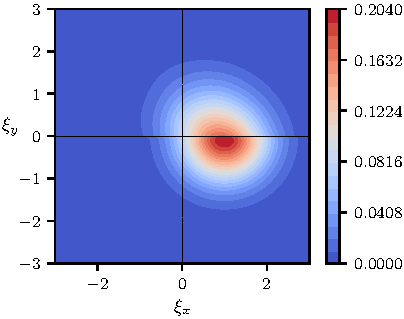
\includegraphics[width=\linewidth]{{{couette/kn0.1-boundary}}}
            \caption{Near the plate \(y=0.4990\)}
        \end{figure}
        \column{.55\textwidth}
        \begin{figure}
            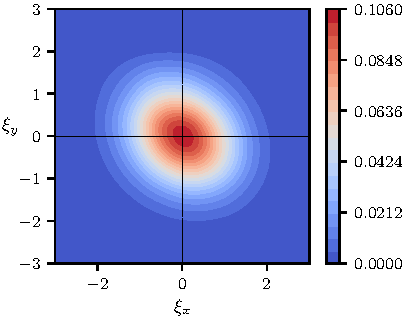
\includegraphics[width=\linewidth]{{{couette/kn0.1-center}}}
            \caption{Near the center \(y=0.0082\)}
        \end{figure}
    \end{columns}
\end{frame}

\begin{frame}
    \frametitle{Distribution function \(\Delta{v}=2\), slice \(\xi_z=0.1665\)}
    \vspace{-20pt} \[ Kn=1 \] \vspace{-20pt}
    \begin{columns}
        \column{.55\textwidth}
        \begin{figure}
            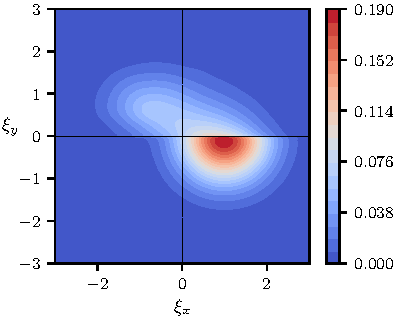
\includegraphics[width=\linewidth]{{{couette/kn1.0-boundary}}}
            \caption{Near the plate \(y=0.4929\)}
        \end{figure}
        \column{.55\textwidth}
        \begin{figure}
            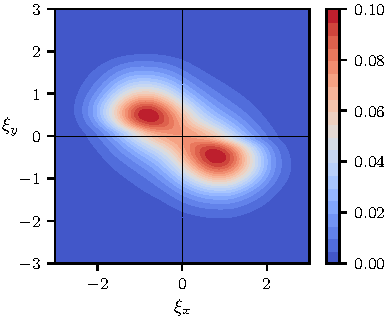
\includegraphics[width=\linewidth]{{{couette/kn1.0-center}}}
            \caption{Near the center \(y=0.0083\)}
        \end{figure}
    \end{columns}
\end{frame}

\begin{frame}
    \frametitle{Distribution function \(\Delta{v}=2\), slice \(\xi_z=0.1665\)}
    \vspace{-20pt} \[ Kn=10 \] \vspace{-20pt}
    \begin{columns}
        \column{.55\textwidth}
        \begin{figure}
            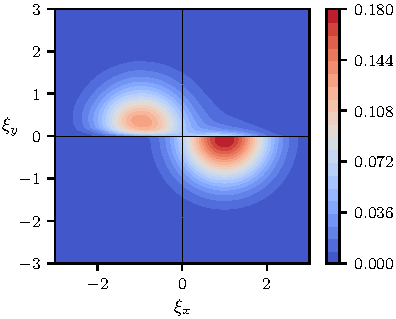
\includegraphics[width=\linewidth]{{{couette/kn10-boundary}}}
            \caption{Near the plate \(y=0.4917\)}
        \end{figure}
        \column{.55\textwidth}
        \begin{figure}
            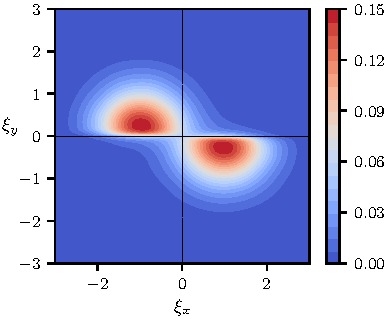
\includegraphics[width=\linewidth]{{{couette/kn10-center}}}
            \caption{Near the center \(y=0.0083\)}
        \end{figure}
    \end{columns}
\end{frame}

\begin{frame}
    \frametitle{Profiles of the longitudinal heat flux}
    \centering
    \includegraphics[width=0.9\linewidth]{couette/qx}
\end{frame}

\begin{frame}
    \frametitle{Profiles of the stress tensor}
    \centering
    \includegraphics[width=0.9\linewidth]{couette/Pzz}
\end{frame}

\begin{frame}
    \frametitle{Shear stress vs \(\Kn\)}
    \vspace{-2pt}
    \centering\hspace{-1.5cm}
    \includegraphics[width=1.1\linewidth]{couette2/shear}
    \hspace{-1.5cm}
\end{frame}

\subsection{Flow between elliptical cylinders}

\begin{frame}
    \frametitle{The velocity field for \(\Kn=0\)}
    \[ T_1 = 1, \quad T_2 = 5.\]
    \centering
    \hspace{-1cm}
    \includegraphics[width=1.1\linewidth]{elliptic/U}
    \hspace{-1cm}
    A nonuniform grid can effective approximate hot and cold gas.\newline
    [Aoki, Sone, Waniguchi 1998]: DSMC simulation for \(0.1 \leq \Kn \leq 5\).
\end{frame}

\begin{frame}
    \frametitle{The velocity field for \(\Kn=0.02\) [Rogozin 2017]}
    \begin{figure}
        \hspace{-.5cm}
        \begin{overprint}
            \onslide<1| handout:3>
                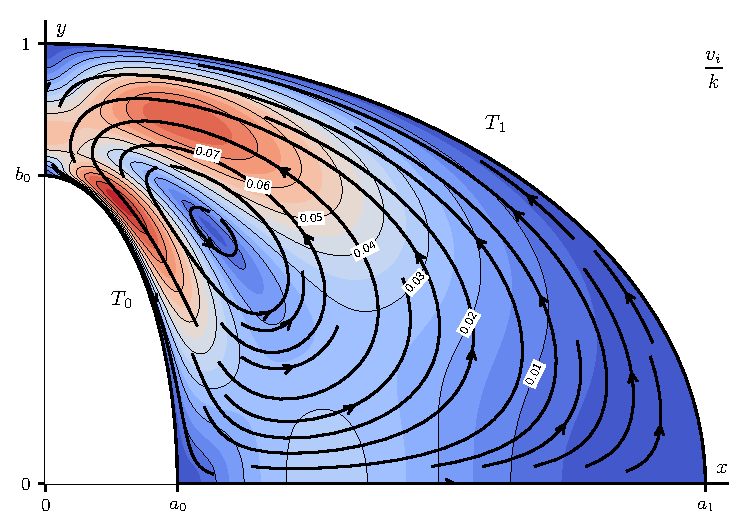
\includegraphics[width=\linewidth]{{{elliptic/kgf-0.02-flow}}}
                \vspace{-20pt}
                \caption{The KGF equations with the \alert{leading}-order boundary conditions}
            \onslide<2| handout:2>
                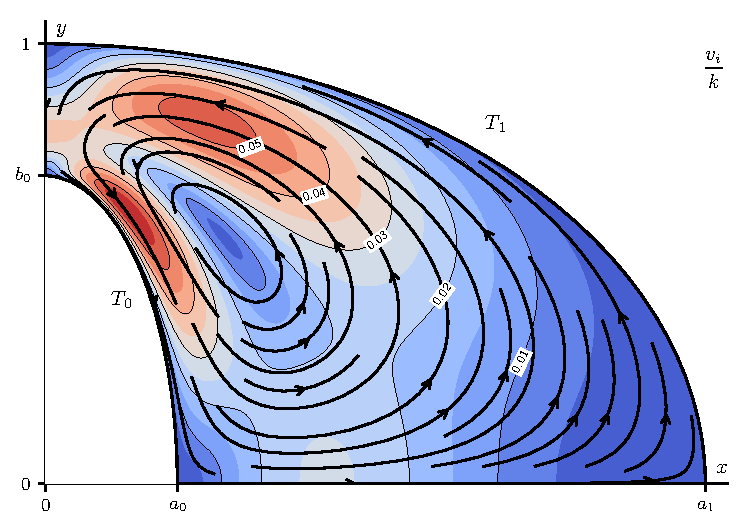
\includegraphics[width=\linewidth]{{{elliptic/first-0.02-flow}}}
                \vspace{-20pt}
                \caption{The KGF equations with the \alert{first}-order boundary conditions}
            \onslide<3| handout:1>
                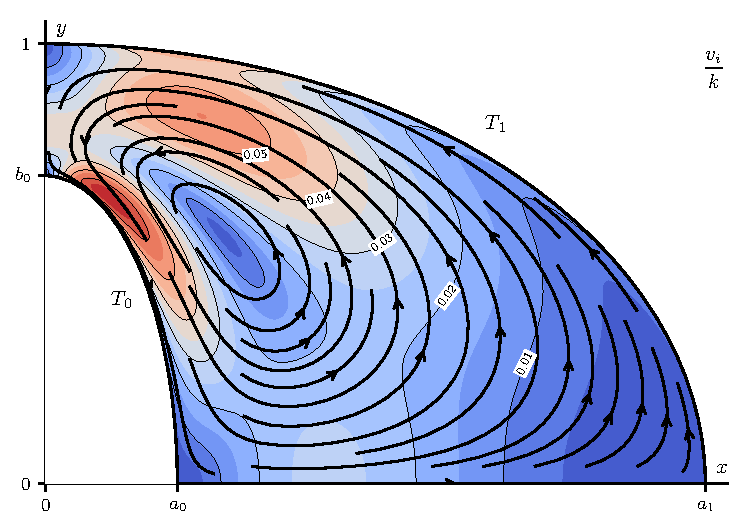
\includegraphics[width=\linewidth]{{{elliptic/second-0.02-flow}}}
                \vspace{-20pt}
                \caption{The KGF equations with the \alert{second}-order boundary conditions\!\!\!\!\!\!\!\!\!}
            \onslide<4| handout:0>
                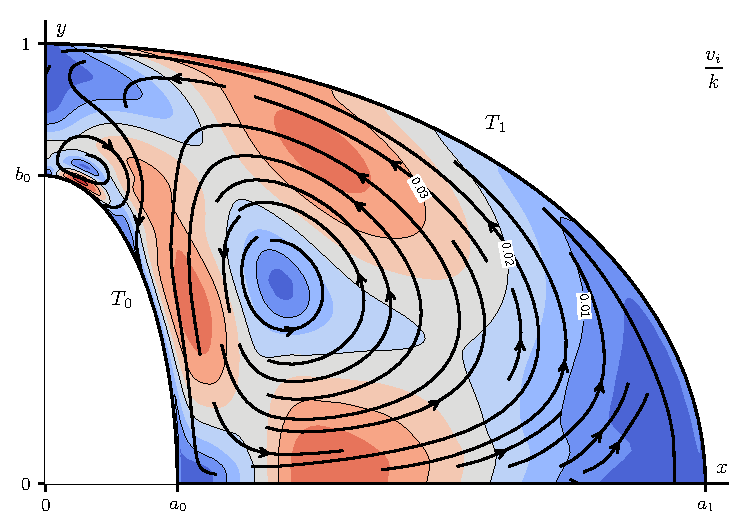
\includegraphics[width=\linewidth]{{{elliptic/kes-0.02-flow}}}
                \vspace{-20pt}
                \caption{Numerical solution of the Boltzmann equation}
        \end{overprint}
    \end{figure}
\end{frame}

\begin{frame}
    \frametitle{Some concluding remarks}
    \begin{itemize}
        \item High-accuracy solutions discover subtle physical effects.
        \item It is worth to study the Knudsen layer carefully, especially physical kinetics in it.
        \item Kogan--Galkin--Friedlander equations can describe the gravity-free thermal-stress convection.
        \item All presented results are obtained on the personal computer.
    \end{itemize}
\end{frame}

\begin{frame}
    \frametitle{References}
    \newcommand\firstdoi{10.1016/j.euromechflu.2016.06.011}
    \newcommand\seconddoi{10.1134/S0965542517060112}
    \newcommand\secondarxiv{1701.05811}
    \begin{itemize}
        \item {[Rogozin 2016]} \\
        “Numerical analysis of the nonlinear plane Couette-flow problem of a rarefied gas for hard-sphere molecules”.
        In:~\textit{European Journal of Mechanics B/Fluids} 60 (2016), pp.~148–163.
        \textsc{doi}:~\href{http://dx.doi.org/\firstdoi}{\alert{\texttt{\firstdoi}}}.
        \item {[Rogozin 2017]} \\
        “Slow non-isothermal flows: numerical and asymptotic analysis of the Boltzmann equation”.
        In:~\textit{Computational Mathematics and Mathematical Physics} 57.7 (2017), pp.~1205–1229.
        \textsc{doi}:~\href{http://dx.doi.org/\seconddoi}{\alert{\texttt{\seconddoi}}}.
        \textsc{arXiv}:~\href{http://arxiv.org/abs/\secondarxiv}{\alert{\texttt{\secondarxiv}}}.
    \end{itemize}
\end{frame}


\end{document}
